
% This is a simple template for a LaTeX document using the "article" class.
% See "book", "report", "letter" for other types of document.

\documentclass[11pt]{article} % use larger type; default would be 10pt

\usepackage[T1]{fontenc}
\usepackage[french]{babel}
\usepackage[utf8]{inputenc} % set input encoding (not needed with XeLaTeX)
\usepackage{kpfonts}

%%% Examples of Article customizations
% These packages are optional, depending whether you want the features they provide.
% See the LaTeX Companion or other references for full information.

%%% PAGE DIMENSIONS
\usepackage{geometry} % to change the page dimensions
\geometry{a4paper} % or letterpaper (US) or a5paper or....
% \geometry{margin=2in} % for example, change the margins to 2 inches all round
% \geometry{landscape} % set up the page for landscape
%   read geometry.pdf for detailed page layout information


% \usepackage[parfill]{parskip} % Activate to begin paragraphs with an empty line rather than an indent

%%% PACKAGES
\usepackage{booktabs} % for much better looking tables
\usepackage{array} % for better arrays (eg matrices) in maths
\usepackage{paralist} % very flexible & customisable lists (eg. enumerate/itemize, etc.)
\usepackage{verbatim} % adds environment for commenting out blocks of text & for better verbatim
% \usepackage{subfig} % make it possible to include more than one captioned figure/table in a single float
% These packages are all incorporated in the memoir class to one degree or another...

%%% HEADERS & FOOTERS
\usepackage{fancyhdr} % This should be set AFTER setting up the page geometry
\pagestyle{fancy} % options: empty , plain , fancy

\usepackage{graphicx} % support the \includegraphics command and options
\usepackage{subcaption}
\usepackage{caption}

\fancyhf{}
\rhead{La Compilation}
\lhead{Optimisation du GCC}
% \rfoot{Page \thepage}
\cfoot{\thepage}

% \renewcommand{\headrulewidth}{0pt} % customise the layout...
% \lhead{}\chead{}\rhead{}
% \lfoot{}\cfoot{\thepage}\rfoot{}

%%% SECTION TITLE APPEARANCE
\usepackage{sectsty}
\allsectionsfont{\sffamily\mdseries\upshape} % (See the fntguide.pdf for font help)
% (This matches ConTeXt defaults)

%%% ToC (table of contents) APPEARANCE
\usepackage[nottoc,notlof,notlot]{tocbibind} % Put the bibliography in the ToC
\usepackage[titles,subfigure]{tocloft} % Alter the style of the Table of Contents
\renewcommand{\cftsecfont}{\rmfamily\mdseries\upshape}
\renewcommand{\cftsecpagefont}{\rmfamily\mdseries\upshape} % No bold!

%%% END Article customizations

%%% The "real" document content comes below...

\title{Optimisation du code par GCC}
\author{Evan VOYLES, Amaury RODRIGUEZ, Stefan GA\L KIEWICZ}
%\date{} % Activate to display a given date or no date (if empty),
         % otherwise the current date is printed

\begin{document}
\maketitle

\section{Notions de compilation}
Il y a une particuliere puissance caché derrière les trois lettres \verb|gcc| - signifiant à la fois
la `Gnu Compiler Collection' et la commande à lancer dans le terminal pour compiler un program C. Enfin pas que.
Quand on appelle une commande de la forme
% { \centering
\begin{verbatim}

    gcc -o hello hello_world.c
\end{verbatim}
on lance effectivement une multitude de processus qui travaillent scrupuleusement en silence.
Il s'agit de:
\begin{enumerate}
    \item Préprocesser le fichier .c
    \item Compiler les fichiers processés pour créer des fichier d'objet (.o)
    \item Relier des fichiers d'objet dans une éxécutable
\end{enumerate}

Ca veut dire quoi, préprocesser un fichier .c ? En effet, à chaque fois qu'on
écrit \verb|#include <stdio.h>| pour inclure un fichier d'entête, avant la compilation
un outil dit le préprocesser va remplacer une ligne d'include avec tout le contenu du fichier d'entête.
Alors la directive préprocesseur \verb|#include| consiste en une opération de copier et coller. Il y a plusieurs d'autres directives qui sont processées avant de compiler,
par exemple le lecteur reconnaitra peut-etre les directives
\begin{verbatim}
    #if, #ifdef, #ifndef, #else, #elif
\end{verbatim}
qui sont employées
pour la compilation conditionnel (par exemple, inclure un fichier spécifique pour Windows si le système est Windows)
où bien pour éviter d'inclure le même fichier plusiers fois:
\begin{verbatim}
    #ifndef MONFICHIER_H
    #define MONFICHIER_H

    / Contenu du fichier monfichier.h /

    ...

    #endif
\end{verbatim}

Après que nos fichiers sont préprocessés, ils sont prêts pour être compilés. La compilation traduit des fichiers en C à des instructions de machine
en binaire, dit des fichiers d'objet qui portent l'extension .o. Pour experimenter chez vous, on peut donner l'option \verb|-c| à gcc pour arrêter après
le compilation et créer des fichiers d'objet.
    Le dernier étape s'agit de regrouper tout les fichiers d'objet pertinents et de les emballer dans une seule exécutable. C'est quoi la différence concrète entre
un `program' C et une `bibliothèque' ? Une bibliothèque c'est une collection des fonctions et leur définitions tandis ce que un program contient la fonction spécial
\verb|main|, qui sert comme une porte d'entrée de l'exécution d'un program.

    Alors finalement l'outil \verb|ld|, dit le `linker' en anglais, relie tous les fichiers .o dans un executable. Son travail est compliqué mais fondamentale. Grosso modo, \verb|ld|
trouve exactement où elle sont définies les fonctions extérieures qu'on appelle dans un program. Par exemple, pour un program simple HelloWorld on va utiliser la fonction \verb|printf| qui
est défini d'ailleurs. Au moment de créer l'exécutable, \verb|ld| va chercher la définition de \verb|printf| dans la bibliothèque standarde et mettre les instructions binaires dans l'exécutable.
La magie de \verb|gcc| c'est qu'il a fait tout cela pour vous en coulisse - un vrai emploi ingrat.

\section{L'Optimisation}
% }
\subsection{-O0}

\subsection{-O1}
\subsection{-O2}
\subsection{-O3}

Your text goes here.

\section{Options Sp\'ecifiques}
Comme on a vu dans le dernier section, il y a de nombreuses options activ\'e avec chaque niveau optimisation et il ne serait pas int\'eressant
de vous d\'enombrer que fait chacun. Donc, on va choisir juste quelques unes \`a \'etudier qui sont utilis\'e souvent

\subsection{Enlever le code superflu}
Pour optimiser le code le compilateur peut enlever du code redondant, en effet le but de l’optimisation du code est de réduire la taille et augmenter la vitesse d’exécution du code.
Une des premières optimisations qui paraît évident est d’enlever le code qui ne sert pas. Il s'agit principalement de deux types du code redondant - dead code (DC, code mort) et dead storage (DS, stockage mort).
Tout segment du code qui ne s'execute pas est dit mort.

\subsubsection{-fdce, -ftree-dce}

\'Etudions le segment du code suivant:
\begin{verbatim}
    if (1 < 2) {
        printf("1 est plus petit que 2");
    } else {
        printf("Ca marche plus les maths");
    }
\end{verbatim}

Ici le compilateur va remarquer qu'il y a un segment de code mort et en d\'eduire que l'on peut optimiser.
Comme nous le voyons dans le code ci-dessus, la condition \verb|1 < 2| est toujours v\'erifi\'e donc la condition du \verb|if| n’a pas
besoin d’être testé et le \verb|else| ne sera jamais exécuté. Vu que la ramification dun programme peut notoirement effectuer des
ralentissements d'\'execution, \verb|gcc| peut enlever la branche \verb|if| et effacer le code mort, sous condition que les options \verb|-fdce| et
\verb|-ftree-dce| soient activ\'ees.

En fait, l'optimisation du code mort est si important que ca que \verb|gcc| enl\`eve automatiquement dans certains cas:
% \begin{figure}
    % \centering
    % \begin{subfigure}[h!]{0.4\textwidth}

\begin{figure}[h!]
    \centering
    \begin{subfigure}[h!]{0.4\textwidth}
        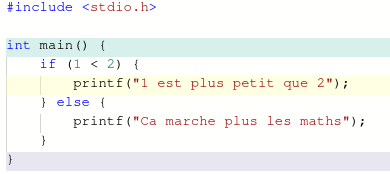
\includegraphics[width=\linewidth]{media/dce_left.png}
        % \subcaption{Code C}
    \end{subfigure}
    \begin{subfigure}[h!]{0.4\textwidth}
        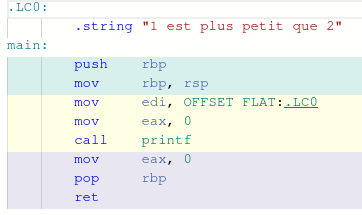
\includegraphics[width=\linewidth]{media/dce-right.png}
        % \subcaption{Assembl\'ee donn\'e par gcc}
    \end{subfigure}
    \caption{Instructions en assembl\'ee gen\'er\'ees pour x86-64 par gcc pour un program simple.}
\end{figure}
N'ayez pas peur de l'assembl\'ee! Comme nous le pouvons constater, les instructions pour la deuxi\`eme branche de l'expression \verb|if| ne sont m\^eme
pas gen\'er\'ees (indiqu\'e par le manque de couleur surlignante l'expression \verb|print|)!

\newpage

On peut comparer cet exemple avec un program simple similaire, mais qui diff\`ere cette fois-ci parce que le compileur ne peut pas d\'eterminer si la condition
est toujours v\'erifi\'e. \'Etudions le program suivant.


\begin{figure}[h!]
    \centering
    \begin{subfigure}[h!]{0.4\textwidth}
        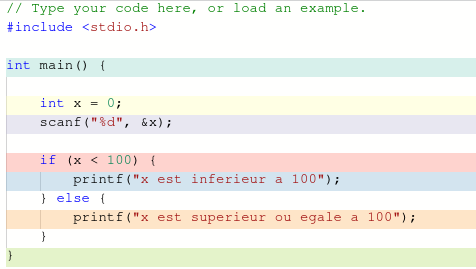
\includegraphics[width=\linewidth]{media/nodfce-left.png}
        % \subcaption{Code C}
    \end{subfigure}
    \begin{subfigure}[h!]{0.4\textwidth}
        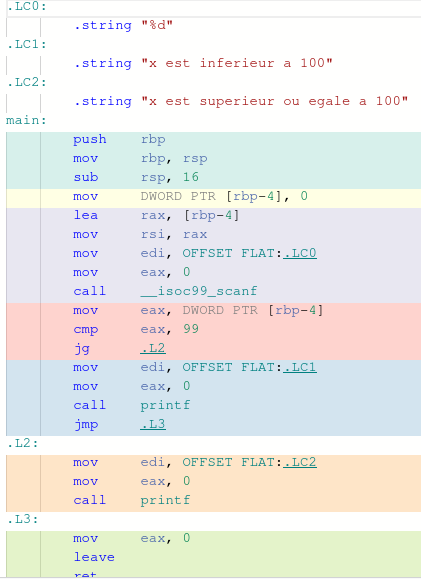
\includegraphics[width=\linewidth]{media/nodce-right.png}
        % \subcaption{Assembl\'ee donn\'e par gcc}
    \end{subfigure}
    \caption{Exemple o\`u des instructions sont gen\'er\'ees pour les deux branches du if}
\end{figure}

Vu que la condition dans le \verb|if| est dependant sur une donn\'ee d'entr\'ee qui se proc\'esse a l'ex\'ecution, il est impossible de d\'eterminer
au moment de compilation si le code est mort. Du coup, il n'y a aucun optimisation dans cet example.


% \begin{minipage}[t]{width=0.5\textwidth}

%     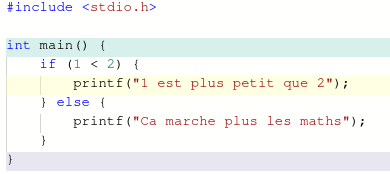
\includegraphics[width=\textwidth]{media/dce_left.png}
% \end{minipage}
    % \end{subfigure}
    % \caption{This is supposed to be a figure}
% \end{figure}

% \begin{minipage}[t]{0.45\textwidth}
% 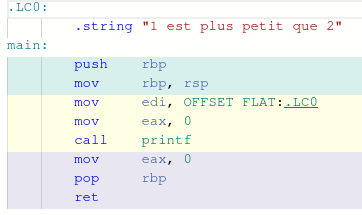
\includegraphics[width=\textwidth]{media/dce-right.png}
% \end{minipage}
% \begin{minipage}[t]{0.45\textwidth}
% 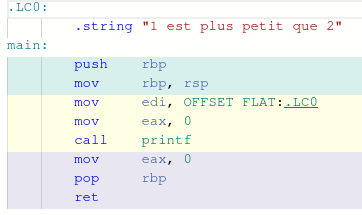
\includegraphics[width=\textwidth]{media/dce-right.png}
% \end{minipage}


% \begin{minipage}[t]{0.3\textwidth}
% 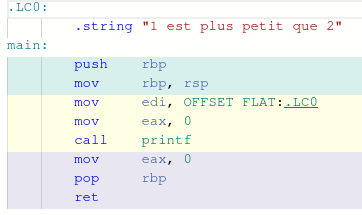
\includegraphics[width=\textwidth]{media/dce-right.png}
% \end{minipage}

\subsubsection{-fdse, -ftree-dse}

Ces options traiten le cas o\`u il y a des variables mortes - c'est-\`a-dire des variables qui ne sont jamais acced\'ees.
Par exemple dans le code qui suit, la variable y n’est pas utilisée. Pour optimiser le code il suffit juste de retirer la ligne et ainsi
réduire la taille et augmenter la vitesse d’exécution du code. Cela marche aussi avec des fonctions qui ne font rien ou ne sont pas utilisés.

\begin{verbatim}

int my_func() {
    int x = 5;
    int y = 5;
    return x;
}
\end{verbatim}

\newpage

On peut \'etudier l'assembl\'e pour visualiser les optimisation fait par gcc.

\begin{figure}[h!]
    \centering
    % \begin{subfigure}[h!]{0.3\textwidth}
    %     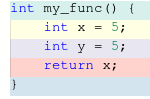
\includegraphics[width=\linewidth]{media/my_func.png}
    %     % \subcaption{Code C}
    % \end{subfigure}
    \begin{subfigure}[h!]{0.4\textwidth}
        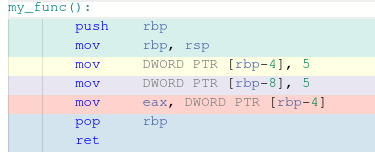
\includegraphics[width=\linewidth]{media/myfuncO0.png}
        \subcaption{-O0}
    \end{subfigure}
    \begin{subfigure}[h!]{0.4\textwidth}
        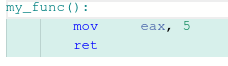
\includegraphics[width=\linewidth]{media/myfuncO1.png}
        \subcaption{-O1}
    \end{subfigure}
    \caption{Exemple o\`u le DSE est enl\`ev\'e}
\end{figure}

La fonction enti\`ere est remplac\'ee par une instruction de charger la valeur 5 dans un registre du CPU.
\end{document}
